\section*{1D analysis of topological states}
In order to have a chiral Hamiltonian I will choose the orientation of the dipoles in a way, such that the chirality remains. This will be done for each lattice configuration separately, i.e. the dipoles depend on the lattice geometry.\\
In order to make the achievement of chirality more feasible I only consider nearest neighbour interactions. When talking of chirality the chirality of the matrix $U$, defined above, is in mind. Recall that
\begin{align*}
    U_{n,m}&=
        -\frac{\partial^2 V_{n,m}(\mathbf{r}_{nm})}{\partial\mathbf{r}_{nm}^2}\quad\text{if}\:n\neq m\\
    U_{n,n} &= \sum_{j;\,j\neq n}\frac{\partial^2 V_{n,j}(\mathbf{r}_{nj})}{\partial\mathbf{r}_{nj}^2}
\end{align*}
Chirality implies that all couplings between sites on the same sublattice vanish. The nearest neighbour restriction already assures that couplings between different sites of the same sublattice vanish. Left is thus only the onsite potential due to the taylor expansion of the dipole dipole potential. The aim is now to choose the orientaiton of the dipoles in such a way that the sum in $U_{n,n}$ is equal to zero.\\ Be aware that so far I didn't write explicitely the dependence of $U$ from the direction of atom movement $x$, $y$. Hence $U_{n,m}$, $U_{n,n}$ are themselves two times two matrixes $(U_{n,m}^{\alpha,\beta})_{\alpha,\beta\in\{x,y\}}$ and the Hamilonian expressed explicitely with respect to the $x$, $y$-phonon modes reads
\begin{align*}
    H &= \sum_{n,\alpha} \omega\,a_{n,\alpha}^\dagger a_{n,\alpha} +\frac{2}{m\omega}\, \sum_{n,m,\alpha,\beta} U^{\alpha,\beta}_{n,m}\,a_{n,\alpha}^\dagger a_{m,\beta}    
\end{align*}
The terms with $a_{n,\alpha}^\dagger a_{n,\alpha}$ can thus be eliminiated by redefining the trap frequency.
\begin{align*}
    \omega_\alpha=\omega+\frac{2}{m\omega}\,U^{\alpha,\alpha}_{n,n}
\end{align*}
Because on the borders $U_{n,n}^{\alpha,\alpha}$ is different from the bulk values, the trap potential for the atoms on the boundary have to be altered to compensate this shift. As I tested in the simulation the existence of separated energies in the bulk band gabs breaks down when the Hamiltonian on the border is different from the bulk.

The terms coupling the two directions of phonon modes on the same side can not be internalized by another quantity. Here the degrees of freedom related to the dipole orientation are exploited to tune the $U_{n,n}^{x,y}$ values to zero, as mentioned above. Because of the nearest neighbour nature of the consideration only two distances play a role, the intracell distance $\mathbf{r}_I$ and the intercell distance $\mathbf{r}_O$. 
\begin{align*}
    U_{n,n}^{x,y}= \frac{\partial^2 V(\mathbf{r}_{I})}{\partial {r}_{I,x}\partial r_{I,y}}+\frac{\partial^2 V(\mathbf{r}_{O})}{\partial {r}_{O,x}\partial r_{O,y}}
\end{align*}
The dipoles are then chosen in such a way that this sum vanishes. For open boundary conditions the values of $U_{n,n}^{\alpha,\beta}$ at the borders are different from the bulk values. In the case of $\alpha=\beta$ the difference can be compensated by changed trap frequencies at the boundary. For the $xy$ coupling this is not possible and the interaction due to both neighboring atoms has to made zero individually such that $x$- and $y$-modes are completely decoupled from each other. \\\\
Informed by simulations where the deviation of the border terms in the Hamiltonian has been kept the topologically non-trivial phase breaks down. It might be at first counter intuitive, that reducing the effect of an open border is decremental to the observation of edge states. It makes, however perfect sense, when remembering that those boundary terms in our case destroy the chrial symmetry. It seems to be neccesarry for the bulk-boundary condition to hold that not only the momentum space Hamiltonian with periodic boundary conditions but also for the real space Hamiltonian with open boundary conditions has to satisfy chiral symmetry. Otherwise one could choose the Hamiltonian describing the border in a completely arbitrary manner and still observe edge states, which would be quite a strong statement.



\subsection*{Aligned dipoles in plane}
I consider a geometry with two sublattices repeating itself in the $x$-axis and separeted by the distance $h$ from each other into the $y$-axis. Different configurations of this geometry are realized by moving the sublattices against each other in the $x$-direction. I consider an even amount of lattice, with $N$ atoms in each sublattice. The $n$th atom of each sublattice $A$ and $B$ takes the position.
\begin{align*}
    \mathbf{r}^A_n&=n\cdot a \,\mathbf{e}_x\\
    \mathbf{r}^B_n&=n\cdot a\, \mathbf{e}_x + b\,\mathbf{e}_x+ h\,\mathbf{e}_y,
\end{align*}
where $a$ is the lattice constant, and the parameters $b$ and $h$ can be chosen to realize different lattice configurations. $b$ and $h$ have to be chosen in a way, such that the nearest neighbor restriction makes sense. 
For any of these geometries there exists a unique orientation of the dipoles which makes the Hamiltonian with periodic boundary conditions chiral.\\\\
By contemplating the spectrum in dependence of the parameter $b$ we find energy state that are well separated from the bulk energy \figref{fig:non_chiral_edge_spectrum}. But the separated energy values converge to a non-zero value, when the number of atoms goes to infinity. But this would be necessary for proper topological edge states. I assume this discrepancy occurs because, as I constructed the dipole moment, the components of the Hamiltonian related to the border are non vanishing. Only the bulk Hamiltonian obeys chiral symmetry. It makes of course sense that the chirality is not only required for the momentum space Hamiltonian with periodic boundary conditions but also for the real space Hamiltonian. In order for the bulk boundary correspondence to hold it seems to be necessary that the real space Hamiltonian satisfies the same symmetries as the momentum space Hamiltonian. Seems reasonable.\\\\
Fortunately it is still possible to set 

\begin{figure}
    \centering
    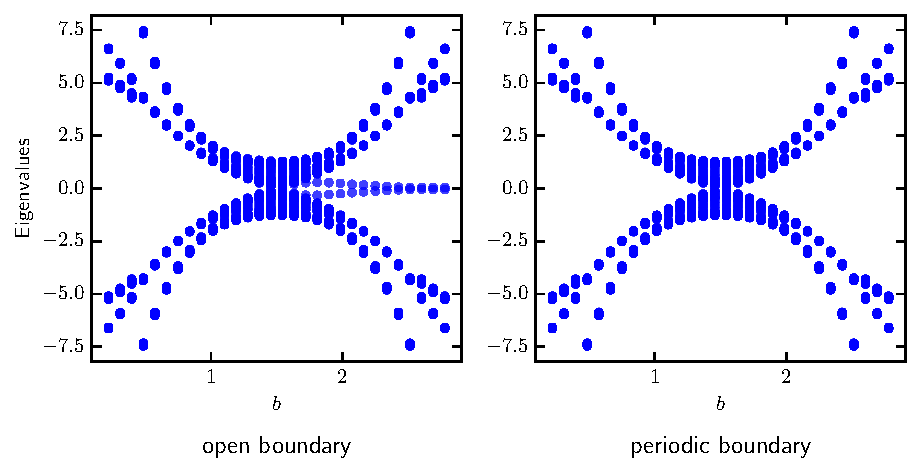
\includegraphics[scale=0.9]{pictures/aligned_dipole_in_plane_sheer_spectrum_h1.1_a3.pdf}
    \caption{\textbf{Spectrum of almost chiral-symmetric Hamiltonian.}}
    \label{fig:non_chiral_edge_spectrum}
\end{figure} 






\begin{figure}
    \centering
    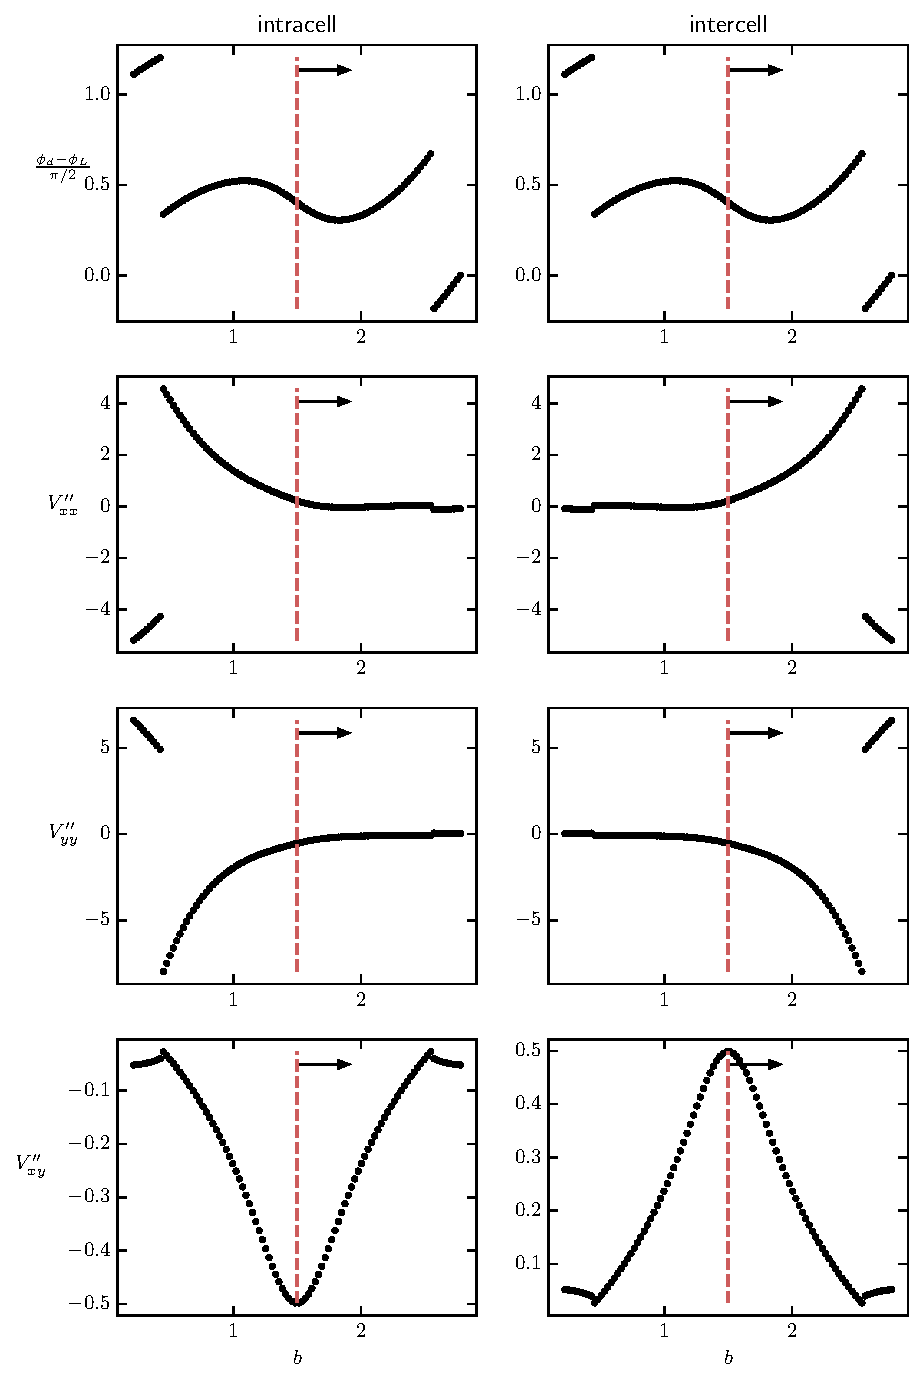
\includegraphics[]{pictures/aligned_dipoles_in_plane_orientation_sheer_h1.1_a3.pdf}
    \caption{The diagram was created with the parameters $a=3$, $h=1.1$. Right to the red dashed line topological phonon states can be found and the winding number is 2.}
\end{figure} 
\begin{figure}
    \centering
    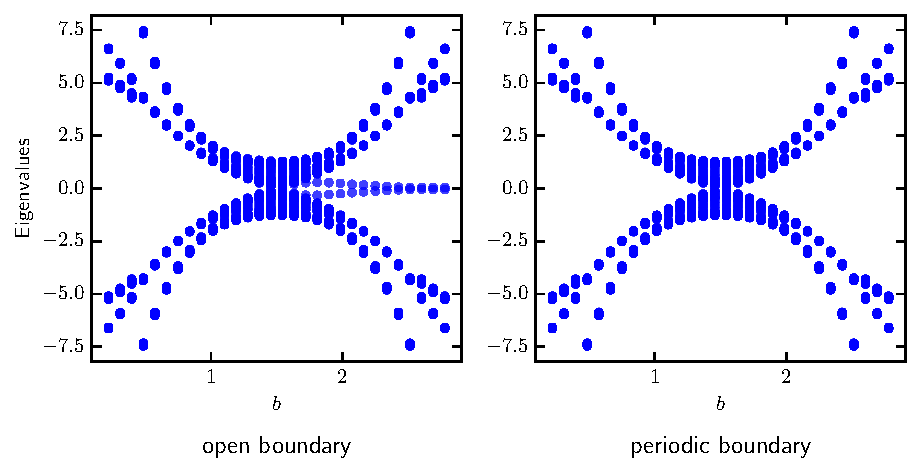
\includegraphics[scale=0.9]{pictures/aligned_dipole_in_plane_sheer_spectrum_h1.1_a3.pdf}
\end{figure} 
\begin{figure}
    \centering
    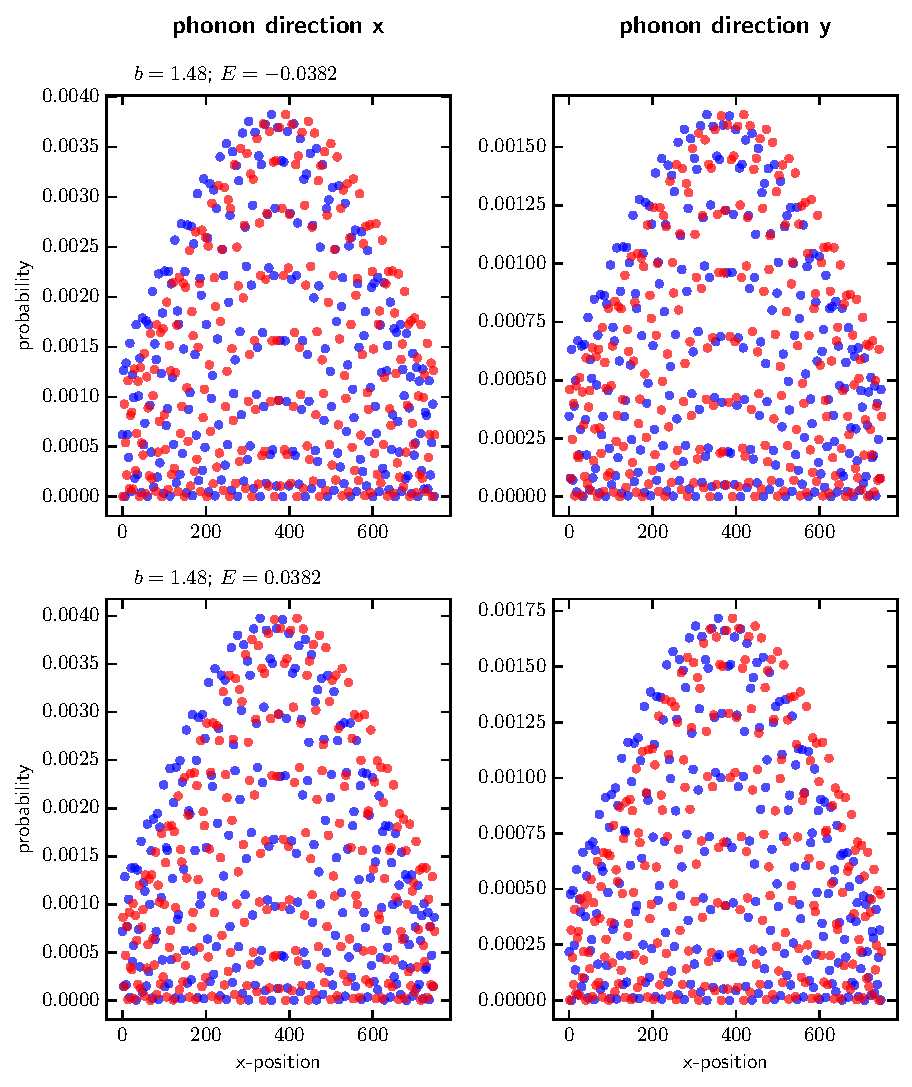
\includegraphics[scale=0.85]{pictures/aligned_dipoles_in_plane_sheer_h1.1_a3_eigenvecs0.pdf}
\end{figure} 
\begin{figure}
    \centering
    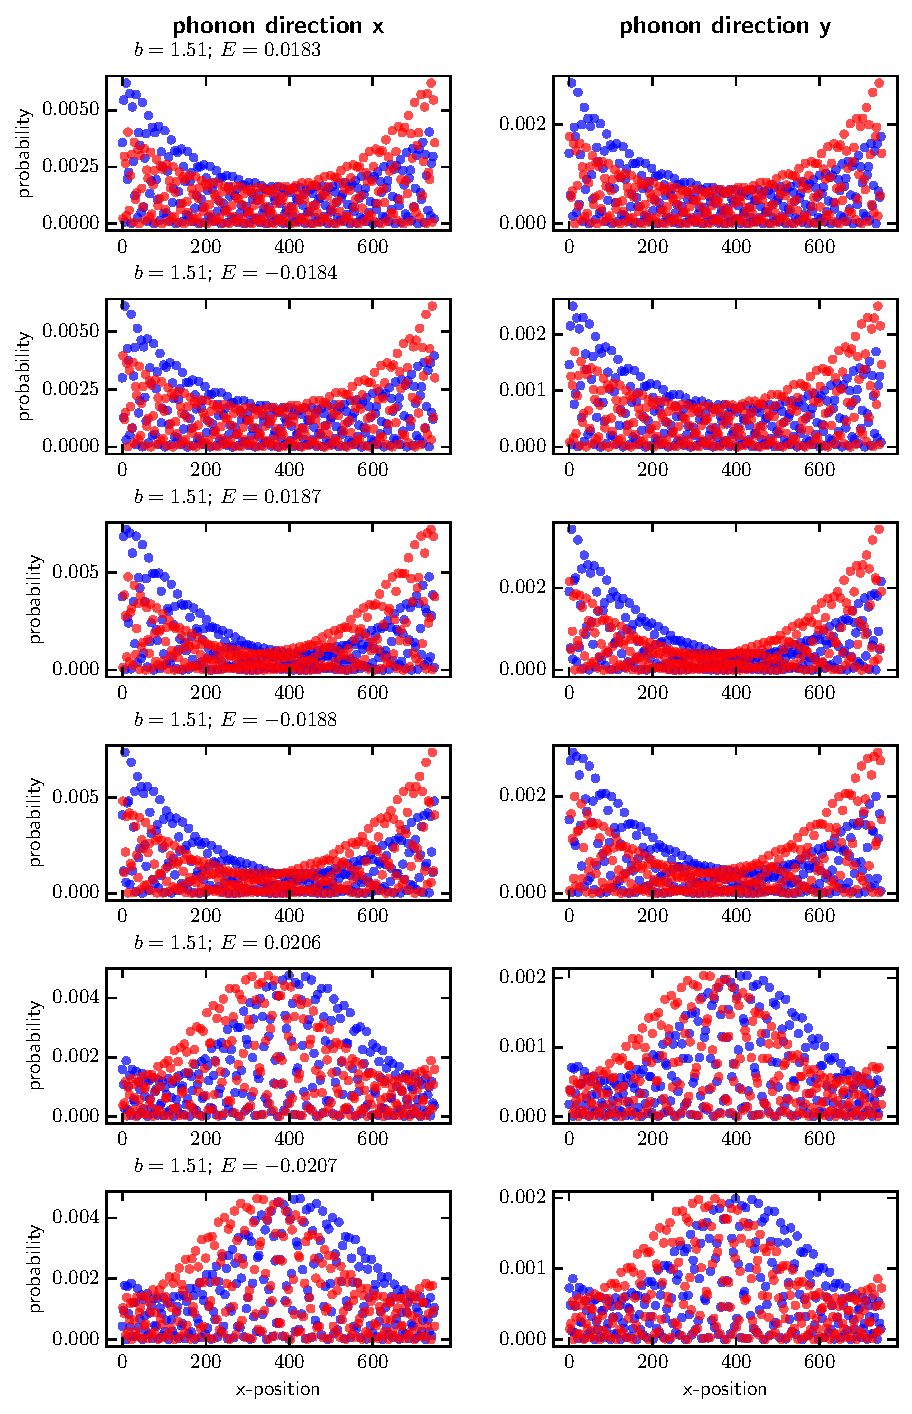
\includegraphics[]{pictures/aligned_dipoles_in_plane_sheer_h1.1_a3_eigenvecs1.pdf}
\end{figure}
\begin{figure}
    \centering
    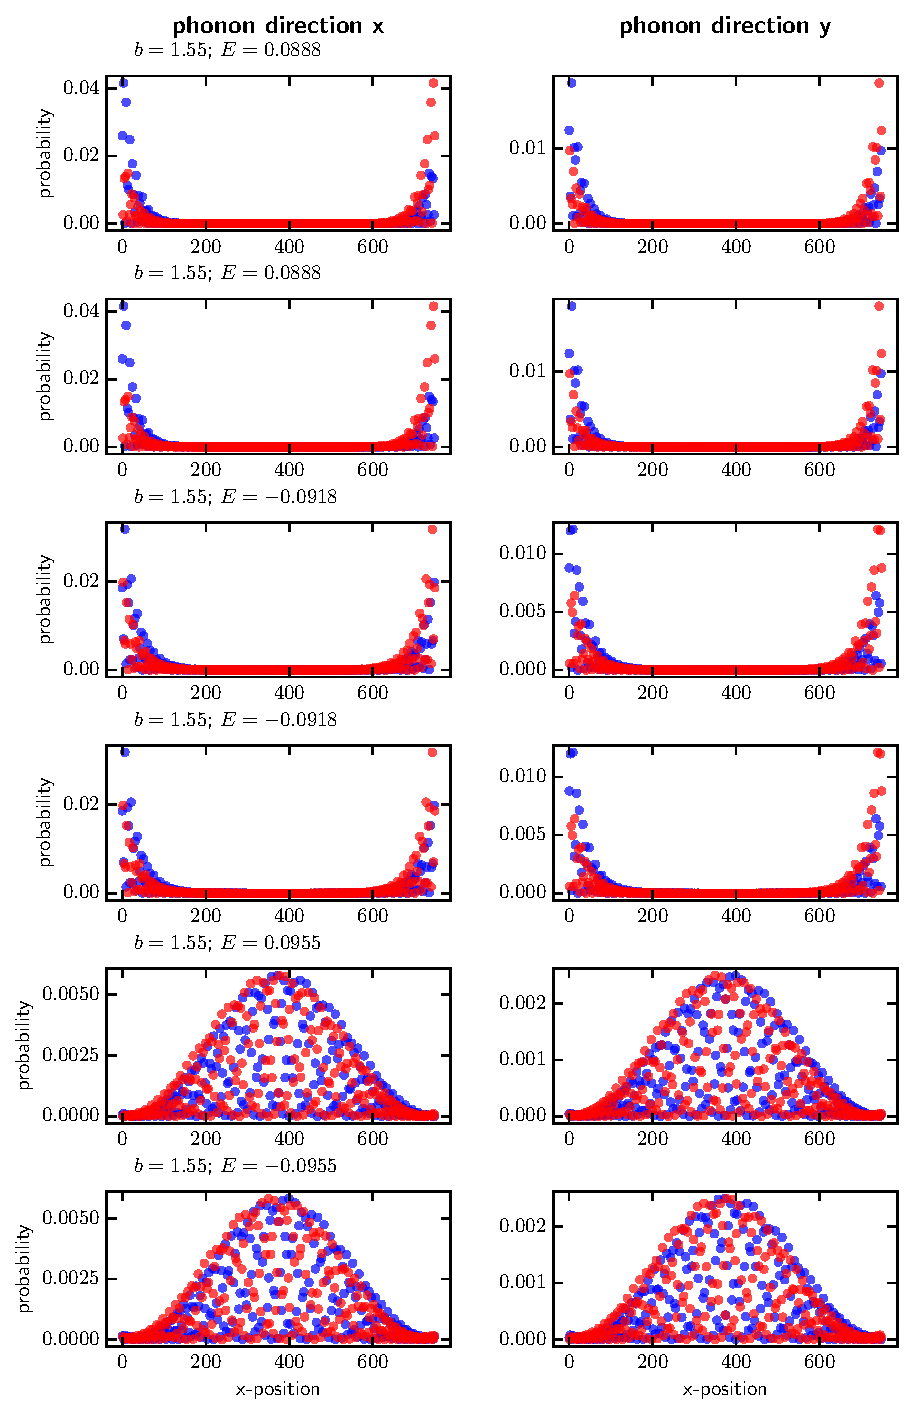
\includegraphics[]{pictures/aligned_dipoles_in_plane_sheer_h1.1_a3_eigenvecs2.pdf}
\end{figure}

\begin{figure}
    \centering
    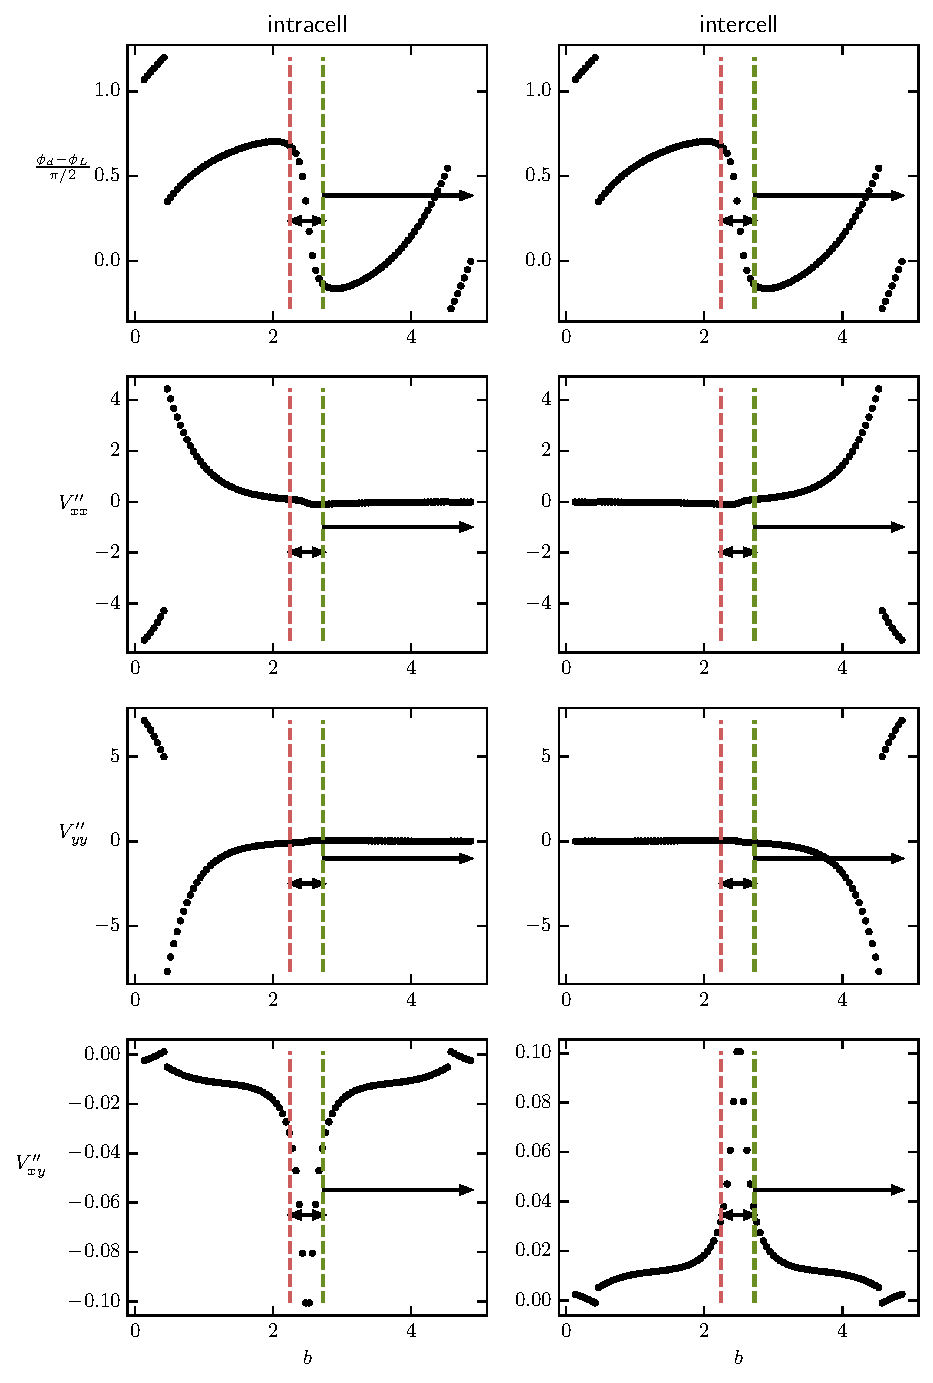
\includegraphics[]{pictures/aligned_dipoles_in_plane_orientation_sheer_h1.1_a5.pdf}
    \caption{The diagram was created with the parameters $a=5$, $h=1.1$. Between the red and the olive dashed line, i.e. bewteen $b$-values of $2.25$-$2.73$ the winding number is 1, whereas right to the olive dashed line the winding number is 2.}
\end{figure} 
\begin{figure}
    \centering
    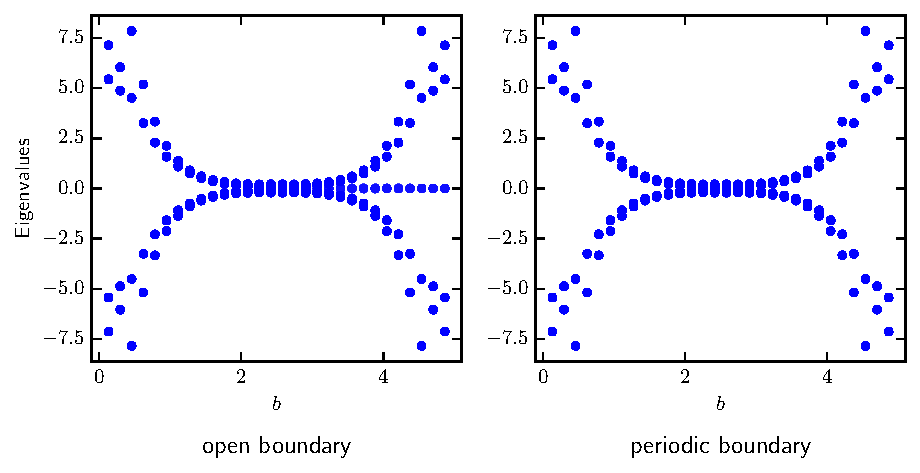
\includegraphics[scale=0.9]{pictures/aligned_dipole_in_plane_sheer_spectrum_h1.1_a5.pdf}
\end{figure} 
\begin{figure}
    \centering
    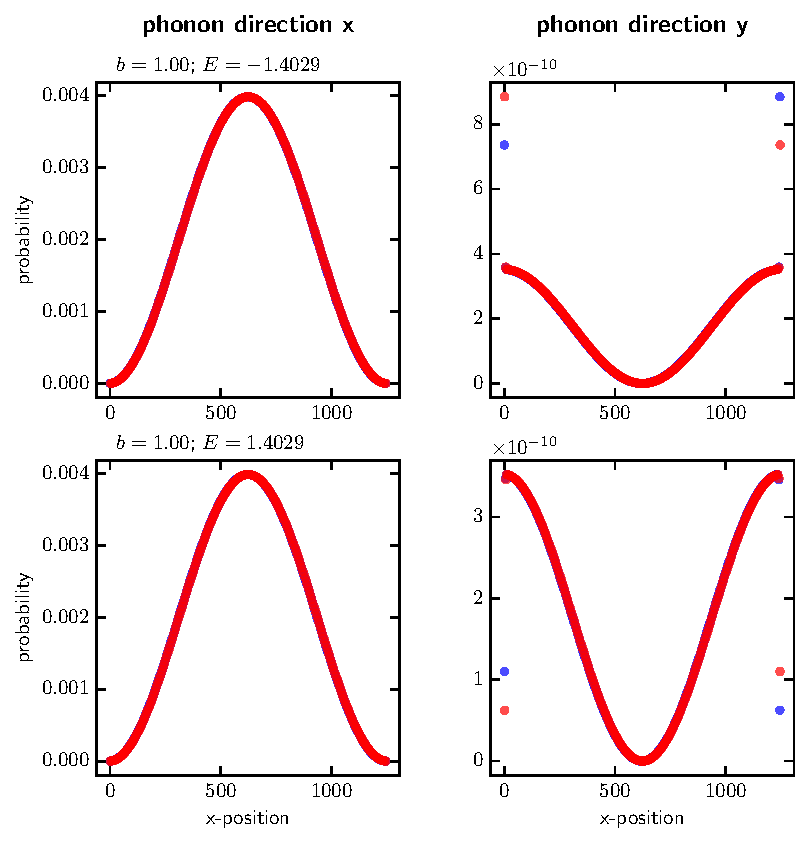
\includegraphics[]{pictures/aligned_dipoles_in_plane_sheer_h1.1_a5_eigenvecs0.pdf}
\end{figure} 
\begin{figure}
    \centering
    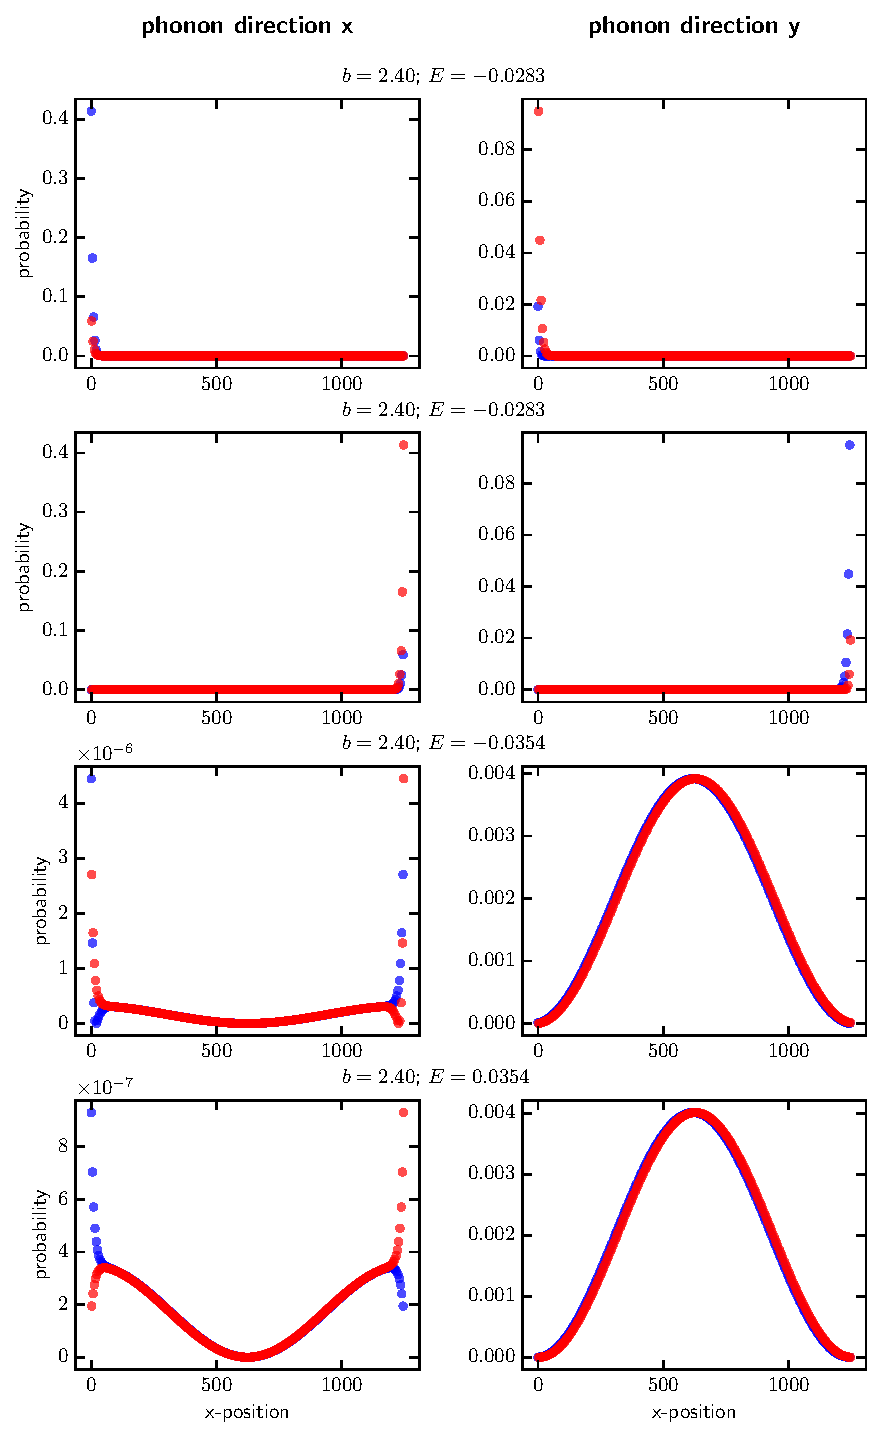
\includegraphics[]{pictures/aligned_dipoles_in_plane_sheer_h1.1_a5_eigenvecs1.pdf}
\end{figure}
\begin{figure}
    \centering
    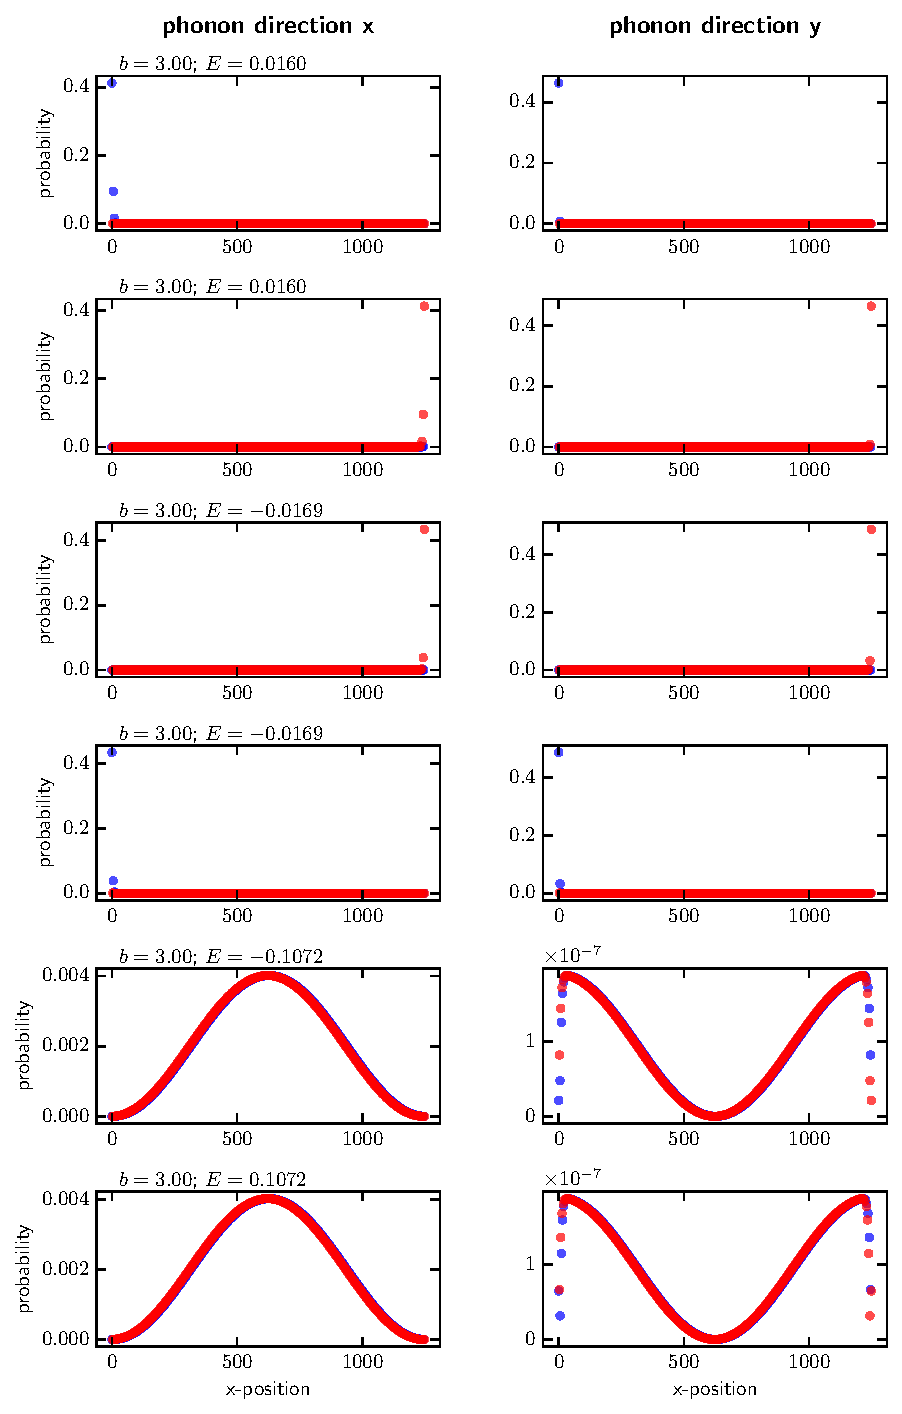
\includegraphics[]{pictures/aligned_dipoles_in_plane_sheer_h1.1_a5_eigenvecs2.pdf}
\end{figure}

% \subsection*{Out of plane dipoles}
% First I will allow the dipoles to point out of the $xy$-plane in which the one dimensional chain will reside. I restrict the dipoles to the following form in order to have easier calcualtions.
% \begin{align*}
%     \mathbf{d}_1= \begin{pmatrix}
%         d_{1,x}\\
%         0\\
%         \sqrt{-d_{1,x}^2}
%     \end{pmatrix},\quad
%     \mathbf{d}_2= \begin{pmatrix}
%         0\\
%         d_{2,y}\\
%         \sqrt{-d_{2,y}^2}
%     \end{pmatrix}
% \end{align*}
% \begin{figure}[H]
%     \centering
%     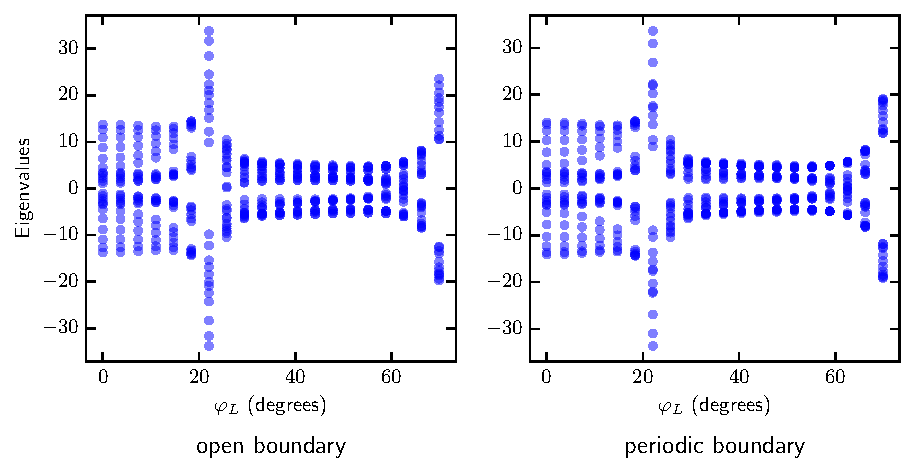
\includegraphics[]{pictures/out_of_plane_dipole_orientation_zigzag.pdf}
% \end{figure}
% \begin{figure}[H]
%     \centering
%     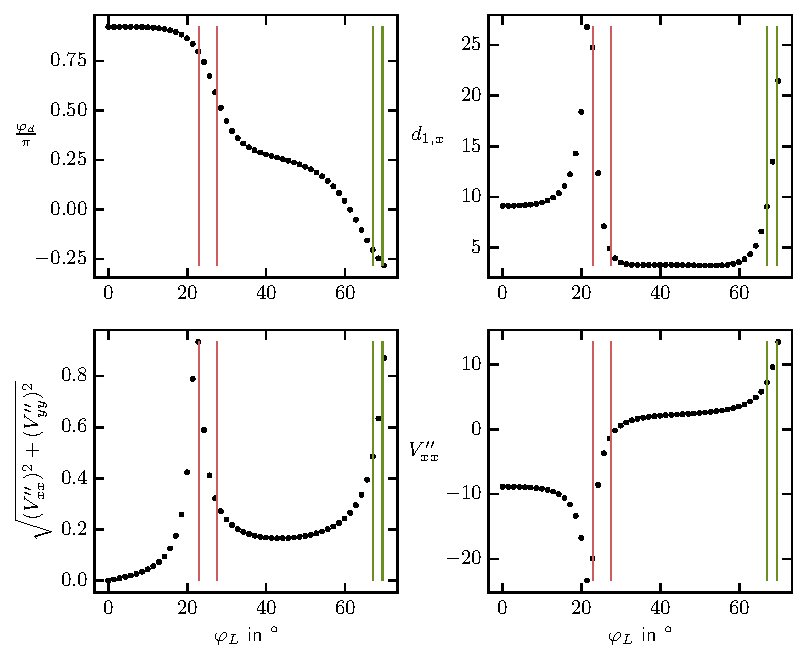
\includegraphics[]{pictures/dipole_orientation_off_plane.pdf}
%     \caption{The occurance of topological states is signaled by the vertical lines. Between the two red as well as between the two green lines topological states can be found.}
% \end{figure}%
% As chain I consider a zig-zag chain with sublattice vector $\mathbf{a}_S$ and lattice vector $\mathbf{a}_L$.
% \begin{align*}
%     \mathbf{a}_S = \begin{pmatrix}
%         c\\
%         \epsilon
%     \end{pmatrix},\quad\mathbf{a}_L = \begin{pmatrix}
%         c+1\\
%         0
%     \end{pmatrix}
% \end{align*}
% For nearest neighbour interaction the condition that lets the momentum space Hamiltonian be chiral under periodic boudary conditions reads
% \begin{align*}
%     0&\overset{!}{=}V''_{xy}(\mathbf{a}_S)+V''_{xy}(\mathbf{a}_S-\mathbf{a}_L)\\
%     V''_{xy}(\mathbf{r}_0)&\vcentcolon=\frac{\partial^2 V}{\partial r_x\partial r_y}(\mathbf{r}_0)
% \end{align*}

% With the particual dipole configuration, introduced above, the derived interaction takes the form
% \begin{align*}
%     V''_{xy}(\mathbf{r})&=d_{1,x}d_{2,y}\,\left( \frac{12}{r^5}-105\,\frac{r_x^2r_y^2}{r^9} \right)+15\,\sqrt{1-d_{1,x}^2}\,\sqrt{1-d_{2,y}^2}\,\frac{r_xr_y}{r^7}\\
%     V''_{\alpha\alpha}(\mathbf{r})&=d_{1,x}d_{2,y}\,\left( 45\,\frac{r_xr_y}{r^7} - 105\,r_\alpha^2\,\frac{r_xr_y}{r^9} \right)+\sqrt{1-d_{1,x}^2}\,\sqrt{1-d_{2,y}^2}\,\left( -\frac{3}{r^5}+15\,\frac{r_\alpha^2}{r^7} \right)
% \end{align*}


% \subsection*{In plane dipole orientation}
% As a next step I restrict the dipoles to the $xy$-plane seperate the magnitude of the dipole projected onto the plane from the occurance of topological states. In this scenario I investigate the properties of the dipole restriction of the following form.
% \begin{align*}
%     \mathbf{d}_1= \begin{pmatrix}
%         d_{1,x}\\
%         d_{1,y}\\
%         0
%     \end{pmatrix},\quad
%     \mathbf{d}_2= \begin{pmatrix}
%         d_2\\
%         0\\
%         0
%     \end{pmatrix}
% \end{align*}
% For this configuration the interaction takes to From
% \begin{align*}
%     V''_{xy}(\mathbf{r})&=d_{1,x}d_2\,\left( 45\,\frac{r_xr_y}{r^7}-105\,\frac{r_x^3r_y}{r^9} \right)+ d_{1,y}d_2\,\left( \frac{12}{r^5}-105\,\frac{r_x^2r_y^2}{r^9} \right)\\
%     V''_{\alpha\alpha}(\mathbf{r})&=d_{1,x}d_2\,\left[ -\frac{3+\delta_{\alpha,x}}{r^5}+\frac{15}{r^7}\,\left( r_x^2 + 2\,r_\alpha r_x+r_\alpha^2+2\delta_{\alpha,x}\,r_x^2\right) -105\,\frac{r_x^2\,r_\alpha^2}{r^9} \right]\\
%     &+ d_{1,y}d_2\,\left[ \frac{15}{r^7}\,\left( r_xr_y + 2\delta_{\alpha,x}\,r_xr_y\right)-105\,\frac{r_\alpha^2r_xr_y}{r^9} \right]
% \end{align*}

% \begin{figure}[H]
%     \centering
%     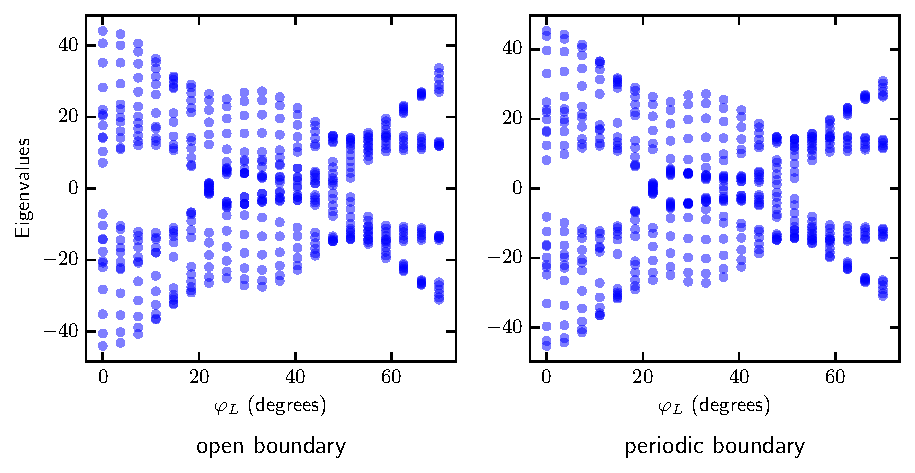
\includegraphics[]{pictures/inplane_dipole_orientation_zigzag.pdf}
% \end{figure} 
% \begin{figure}[H]
%     \centering
%     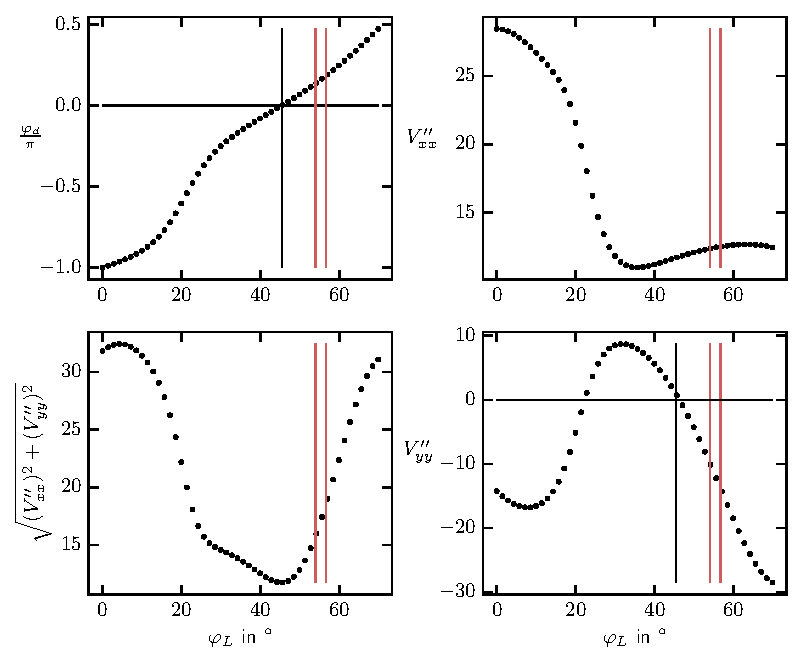
\includegraphics[]{pictures/dipole_orientation_in_plain.pdf}
%     \caption{Topological states can again be found in the angle range between the two red vertical lines.}
% \end{figure}

% \subsection*{1D hexagonal chain}
% In this chapter I consider a chain with equal spacing $r$ between the atoms where the angle $\varphi$ is changed in a manner, such that the first layer of a 2D hexagonal lattice is reached. Because of the one dimensionality of the chain the unit cell contains four atoms (A, B, C, D).
% \begin{align*}
%     \mathbf{a}_L&=\begin{pmatrix}
%         2r\,(1+\cos\varphi_L)\\0
%     \end{pmatrix}\quad\mathbf{a}_B=\begin{pmatrix}
%         r\cos\varphi_L\\r\sin\varphi_L
%     \end{pmatrix}\\
%     \mathbf{a}_C&=\begin{pmatrix}
%         r\,(1+\cos\varphi_L)\\r\sin\varphi_L
%     \end{pmatrix}\quad\mathbf{a}_D=\begin{pmatrix}
%         r\,(1+2\cos\varphi_L)\\0
%     \end{pmatrix}
% \end{align*}

% \begin{figure}
%     \centering
%     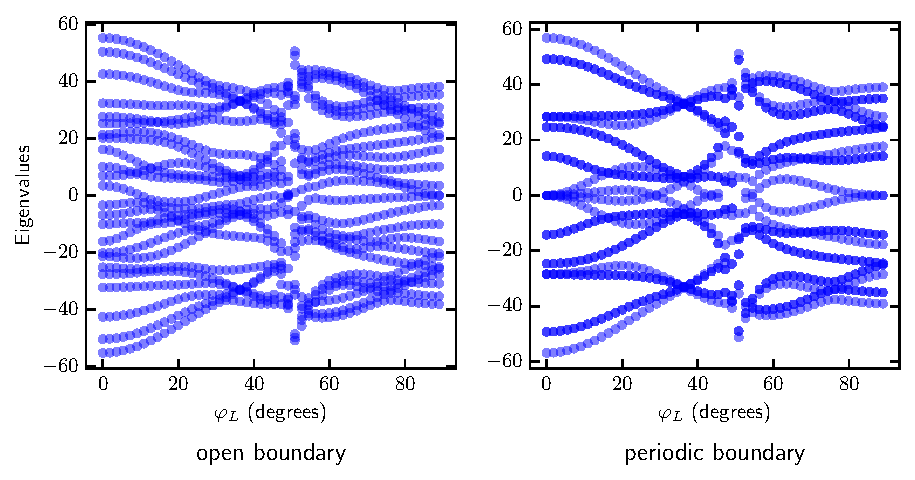
\includegraphics[]{pictures/in_plane_dipole_orientation_hex1D.pdf}
% \end{figure} 
% \begin{figure}
%     \centering
%     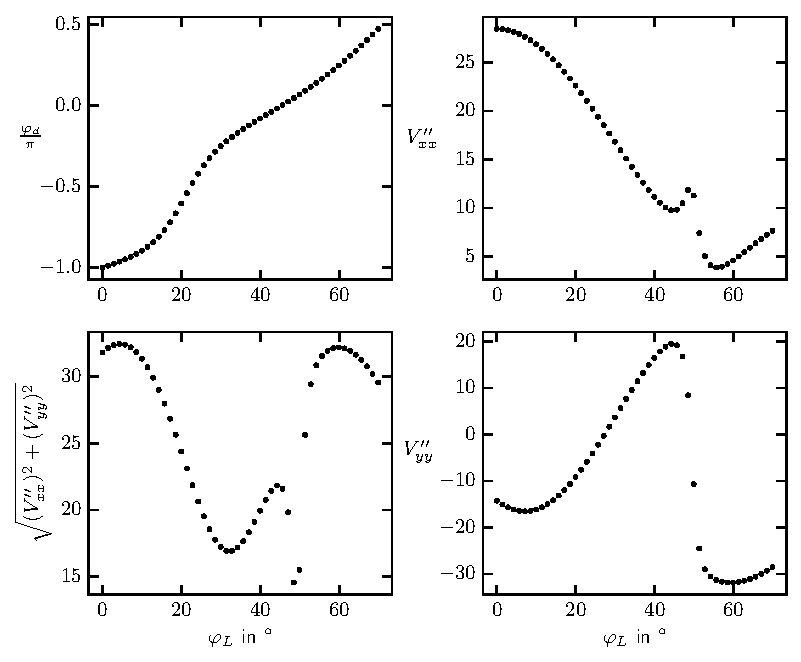
\includegraphics[]{pictures/dipole_orientation_in_plane_hex1D.pdf}
%     \caption{In this configuration with equal spacing between the atoms no topological states occur.}
% \end{figure}

% \section{Aligned dipoles in plane}
% \begin{figure}
%     \centering
%     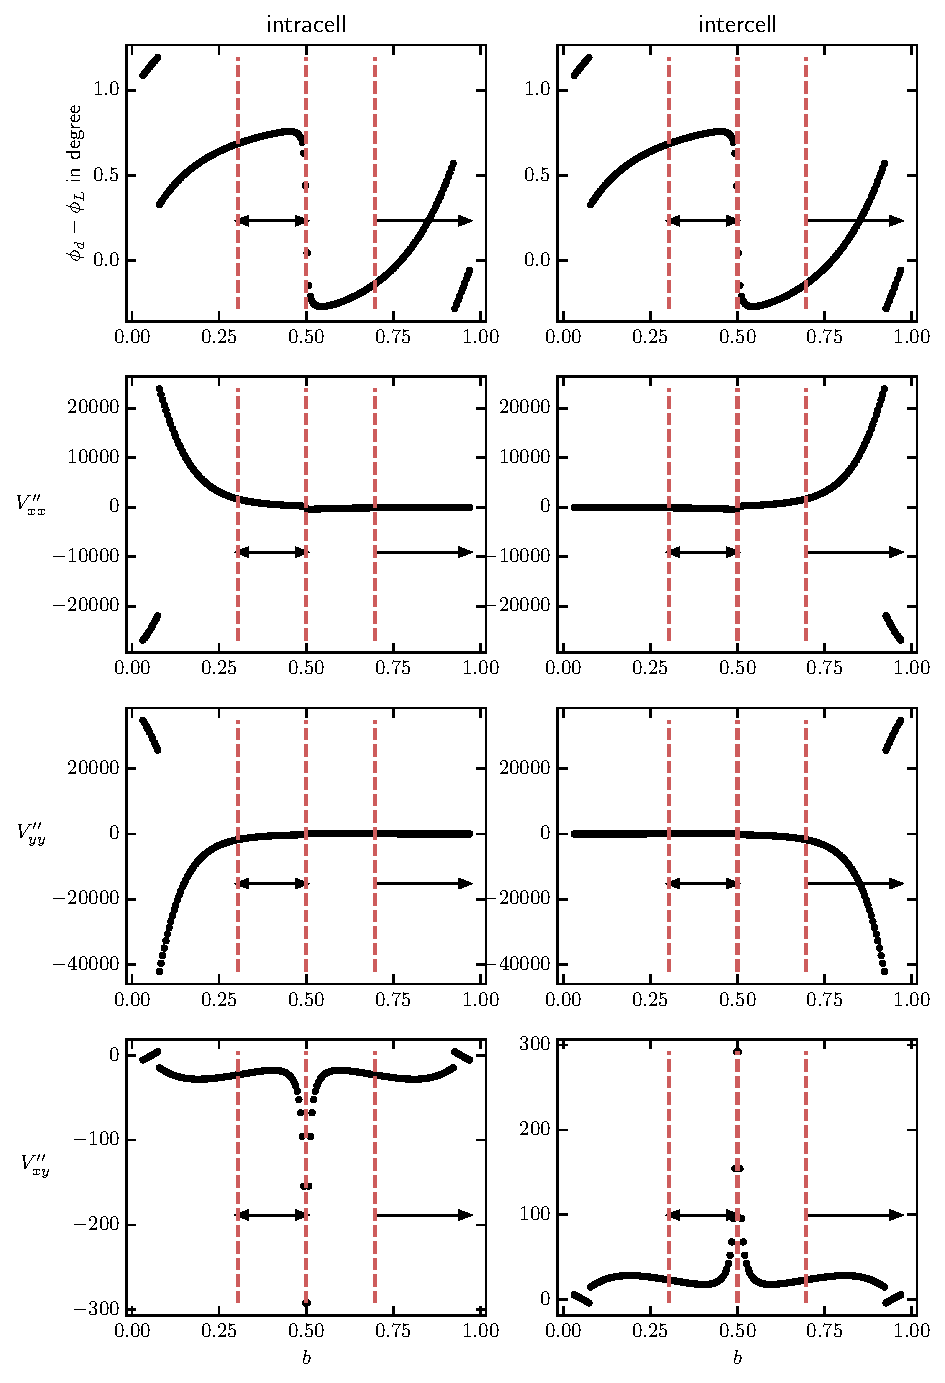
\includegraphics[]{pictures/aligned_dipoles_in_plane_zigzag_h0.2.pdf}
% \end{figure} 
% \begin{figure}
%     \centering
%     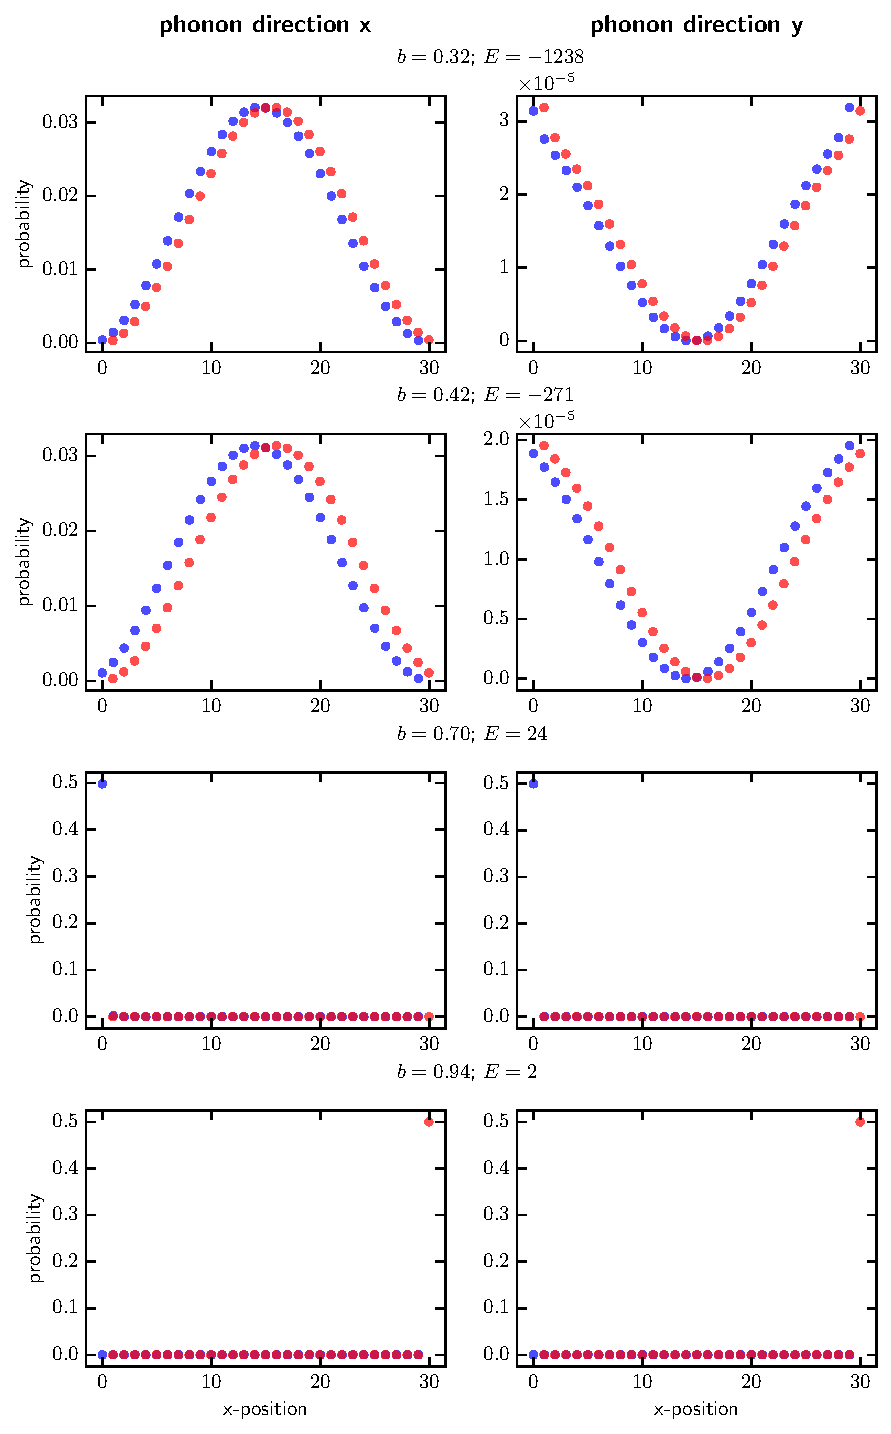
\includegraphics[]{pictures/aligned_dipoles_in_plane_zigzag_h0.2_eigenvecs.pdf}
% \end{figure} 
% \begin{figure}
%     \centering
%     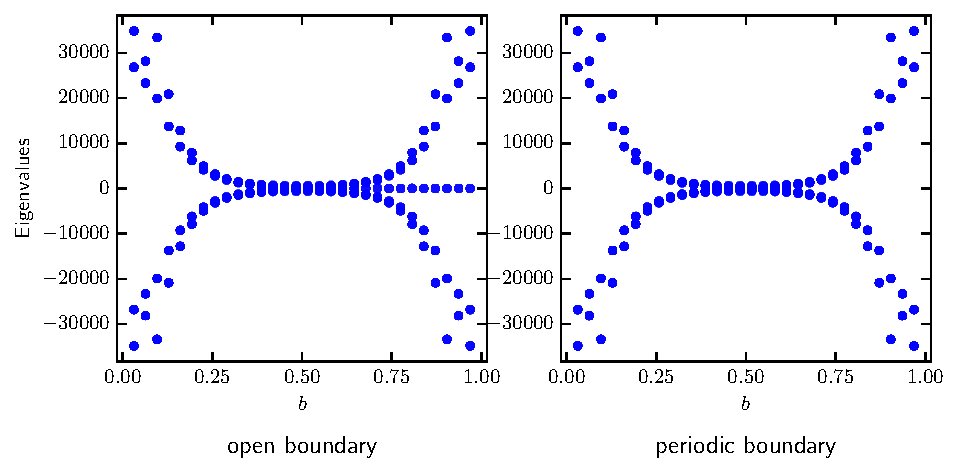
\includegraphics[]{pictures/aligned_dipole_in_plane_zigzag_spectrum_h0.2.pdf}
% \end{figure} 
% \begin{figure}
%     \centering
%     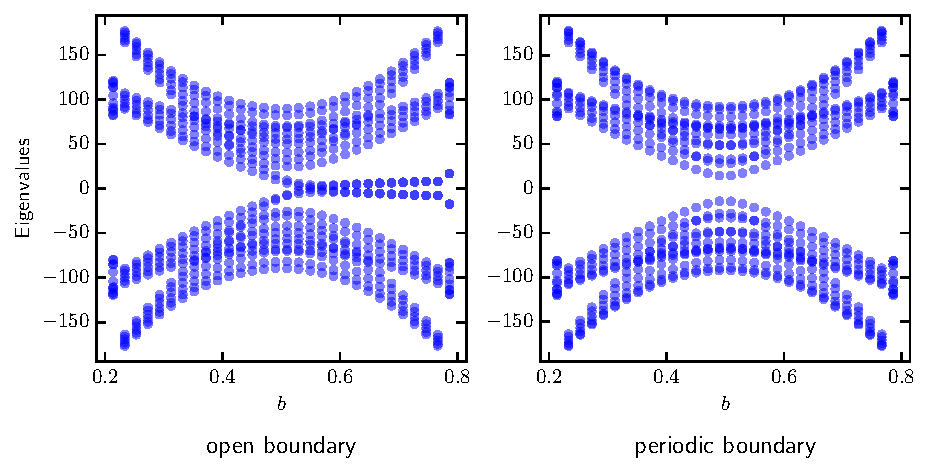
\includegraphics[]{pictures/aligned_dipole_in_plane_zigzag_spectrum_h0.6.pdf}
% \end{figure} 
% \begin{figure}
%     \centering
%     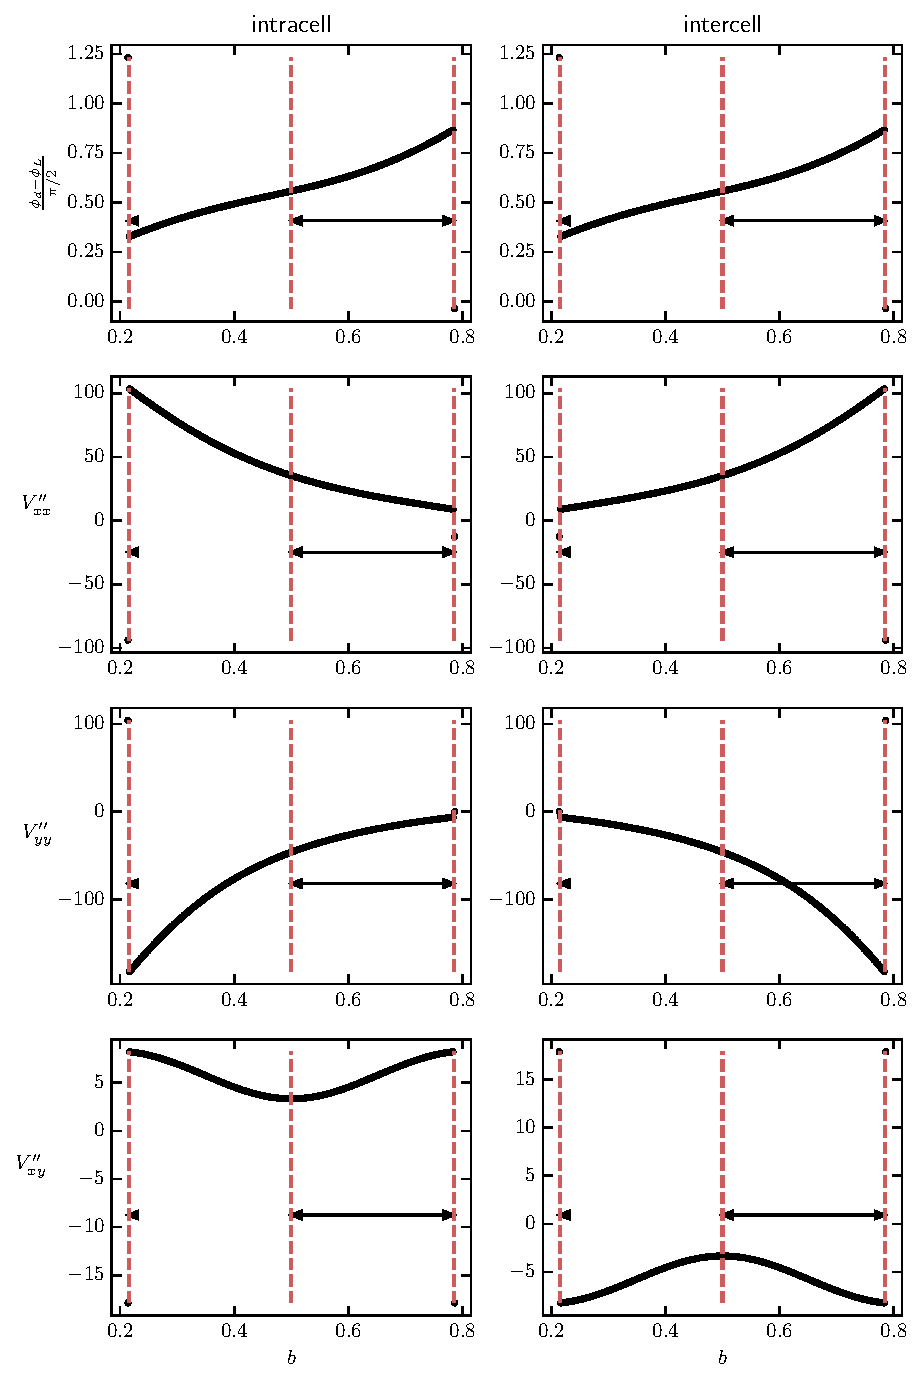
\includegraphics[]{pictures/aligned_dipoles_in_plane_zigzag_h0.6.pdf}
% \end{figure} 
% \begin{figure}
%     \centering
%     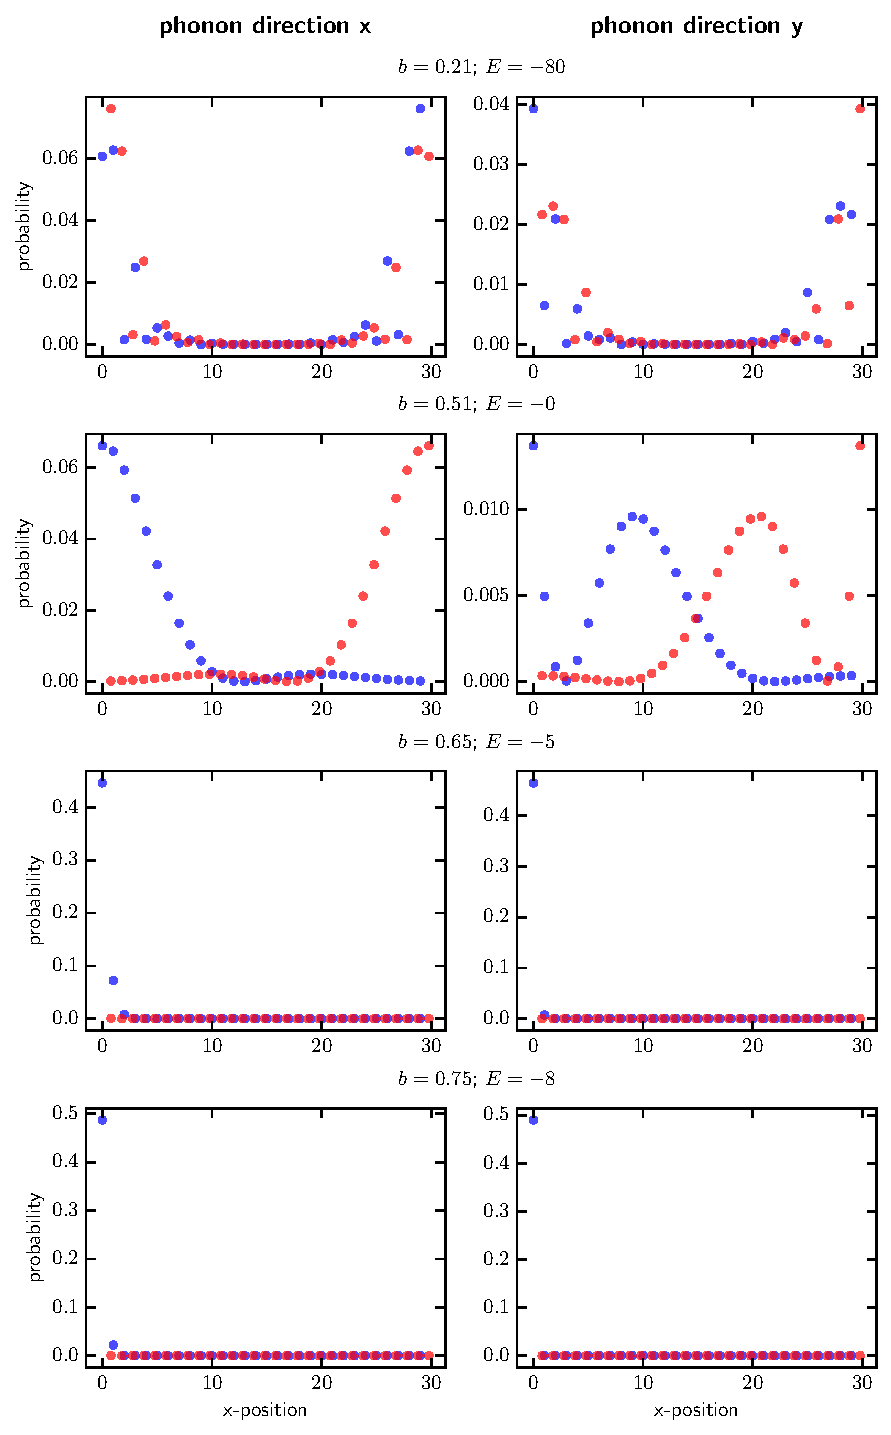
\includegraphics[]{pictures/aligned_dipoles_in_plane_zigzag_h0.6_eigenvecs.pdf}
% \end{figure} 

